\documentclass{article}
\usepackage[utf8]{inputenc}
\usepackage{subfig}

%References
\usepackage{natbib}
%IMPORTANT use https://www.citationmachine.net/ if you need to generate references!
% \citep{reference} creates Harvard Style references throughout

%Colors
\usepackage{xcolor}

\usepackage[protrusion=true,expansion]{microtype}

%Code Markup
\usepackage[outputdir=cache]{minted}
%Syntax Highlighting Style
\definecolor{bggray}{RGB}{40,40,40}
%Macro to make a Syntax Highlighter For Java files 
%Use \javacode{filename.java} to insert a Java File W/ Syntax Highlighting file into the PDF
\newmintedfile[javacode]{java}{
	style=fruity,
	bgcolor=bggray,
	linenos,
	breaklines,
	tabsize=2,
	obeytabs
}

\newmintedfile[bashoutput]{txt}{
	style=fruity,
	bgcolor=lightgray,
	breaklines,
	tabsize=2,
	obeytabs
}

\newmintedfile[racketcode]{racket} {
	style=fruity,
	bgcolor=bggray,
	breaklines,
	tabsize=2,
	obeytabs
}

%Page Margins and stuff
\usepackage{geometry}
 \geometry{
 a4paper,
 total={170mm,257mm},
 left=20mm,
 }

%Pictures
\usepackage{graphicx}
\graphicspath{ {./images/} }

%Move the title position
\usepackage{titling}

\setlength{\droptitle}{-8.5em} %Up, near the top but not too high

\title{CT331 Assignment 2}
\author{Daniel Hannon (19484286)}
\date{November 2021}

\begin{document}
	\maketitle
	\section{Question 1}
		\subsection{Code}
			\racketcode{question1.rkt}
		\subsection{Output}
			\begin{figure}[h!]
				\centering
				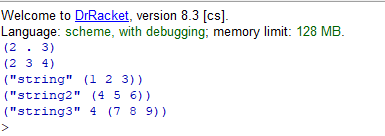
\includegraphics[width=0.7\textwidth]{1}
			\end{figure}
		\subsection{Part B}
			Cons, when passed two atomics creates a list with the dot to indicate where car returns (the left) and where cdr returns (the right)\\
			If you pass a List as the first or second parameter it no longer features the dot.\\
			In order to feature a list within it, you must encase the list within another set of brackets.\\
			With List you do not need to do this .\\
			With append you cannot pass atomics so everything must be passed as a list.
			
		\newpage
	\section{Question 2}
		\subsection{Code}
			\racketcode{question2.rkt}
			\newpage
		\subsection{Output}
			\begin{figure}[h!]
				\centering
				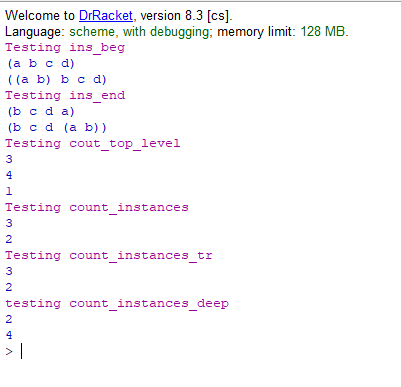
\includegraphics[width=0.7\textwidth]{2}
			\end{figure}
		\newpage
	\section{Question 3}
		\subsection{Code}
			\racketcode{question3.rkt}
		\subsection{Output}
			\begin{figure}[h!]
				\centering
				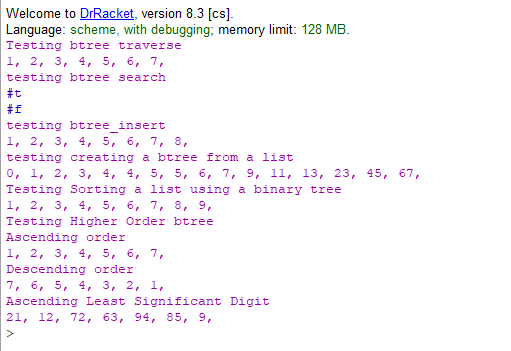
\includegraphics[width=0.7\textwidth]{3}
			\end{figure}
	%Sets to Harvard Style and links the references file
	\bibliographystyle{agsm}
	\bibliography{references}
\end{document}